\phantomsection
\addcontentsline{toc}{part}{Physics Past Papers}
\part*{Physics Past Papers} \index{Past Papers!Physics}
\label{cha:past-papers-phys}


%\titlespacing*{\chapter}{0pt}{-50pt}{20pt}
%\titleformat{\chapter}[display]{\normalfont\huge\bfseries}{\chaptertitlename\
%\thechapter}{20pt}{\Large}

%\chapter{NECTA Past Papers - Physics}

%\pagebreak

\setcounter{secnumdepth}{0}
\index{Past Papers!Physics!2013}
\chapter{2013 - PHYSICS 2A ACTUAL PRACTICAL A}

\begin{enumerate}
\item[1.] You are provided with a metre rule, a knife edge, two strings of length 100 cm each and two weights $W_1$ and $W_2$ of masses 50 g and 100 g respectively. Proceed as follows:
\begin{enumerate}
\item[(a)] Balance a metre rule on a knife edge, put a mark and write G at the balancing point using a piece of chalk or a pencil. Measure and record the length $l$, width $w$ and thickness $t$ of a metre rule using a vernier caliper.
\item[(b)] Place the metre rule on a knife edge so that the knife edge is at 60 cm of your metre rule (see Figure 1 (a)). Suspend weight $W_2$ of 100 g on the right hand side of the knife edge. Adjust $W_2$ until the metre rule balances horizontally. Read and record lengths `b' and `c' as seen in Figure 1 (a).

\begin{center}
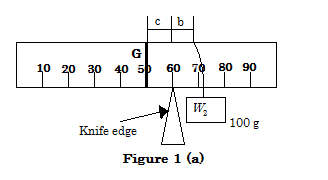
\includegraphics[width=9cm]{./img/2013-1a-alt.png}
\end{center}

\begin{enumerate}
\item[(i)] Suspend weight $W_1$ of 50 g on the left hand side of the knife edge at the position 47 cm and adjust weight $W_2$ until the metre rule balances horizontally as seen in Figure 1 (b). Read and record the lengths `a' and `b'.

\begin{center}
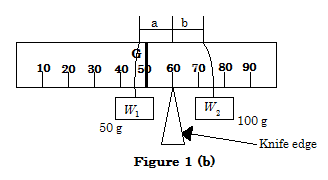
\includegraphics[width=9cm]{./img/2013-1b-alt.png}
\end{center}

\item[(ii)] Repeat the procedures in (b) (i) by adjusting the position of $W_1$ to the left at the interval of 3 cm to obtain other four (4) readings.
\end{enumerate}
\item[(c)] Tabulate your results as shown in Table 1.\\

\quad Table 1\\
\quad \quad \begin{tabular}{|p{4cm}|p{4cm}|} \hline
\multicolumn{1}{|c|}{a (cm)} & \multicolumn{1}{c|}{b (cm)} \\ \hline
& \\ \hline
& \\ \hline
\end{tabular}\\[10pt]

\item[(d)] Plot a graph of ``b'' against ``a''.
\item[(e)] What is the nature of the graph?
\item[(f)] Calculate the slope $S$ of the graph.
\item[(g)]
\begin{enumerate}
\item[(i)] Read the $b$-intercept, given that $b = Sa + \cfrac{W}{W_2} \times c$
\item[(ii)] What does $\left(\cfrac{W}{W_2}\right)c$ represent in your graph?
\item[(iii)] Calculate the value of $W$ using the relation $W_2 = \cfrac{Wc}{9.5 \text{cm}}$. What does $W$ represent?
\end{enumerate}
\item[(h)]
\begin{enumerate}
\item[(i)] Find the value of the ratio $P = \cfrac{l \times w \times t}{m}$.
\item[] \textbf{Note:} The mass $m$ of a meter rule can be obtained by calculations.
\item[(ii)] What is the physical meaning of the value of $P$?
\end{enumerate}
\item[(i)] State a possible source of error in this experiment.
\item[(j)] How can you minimize error in 1 (i)?
\item[(k)] State the aim of this experiment.
\end{enumerate}
\end{enumerate}
\flushright \textbf{(25 marks)}
\flushleft

\begin{enumerate}
\item[2.] You are provided with a Plane mirror, a Ruler, Protract, Drawing board, Optical pins, Office pins and Plain papers. Proceed as follows:
\begin{enumerate}
\item[(a)] On the plain paper provided, draw a line 13 cm from the top of the paper and call it M$_1$M$_2$. Pin your paper on the board provided and place the reflecting surface of the mirror along the line M$_1$M$_2$ as seen in Figure 2.

\begin{center}
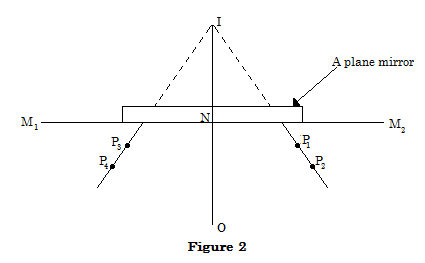
\includegraphics[width=10cm]{./img/2013-2-alt.png}
\end{center}

\item[(b)] Insert pin O as an object at 4.0 cm in front of the mirror. Place pins P$_1$ and P$_2$ so as to appear in one straight line with the image of object O seen in the plane mirror.
\item[(c)] Remove pins P$_1$ and P$_2$, using other pins, place pins P$_3$ and P$_4$ so as to appear in a straight line with the image of object O in the other side (see Figure 2).
\item[(d)] Remove the mirror and pins. Draw lines joining P$_1$ and P$_2$ on one side and the other joining P$_3$ and P$_4$ on the other side of object O, extend both lines to meet at I on the other side of line M$_1$M$_2$.
\item[(e)] Join OI, a line cutting the reflecting surface at N.
\item[(f)] Repeat this procedure for the distance of an object being 6, 8, 10 and 12 cm.
\item[(g)] On all the diagrams drawn:
\begin{enumerate}
\item[(i)] Measure the distance ON and NI.
\item[(ii)] Comment on the distances obtained in 2 (g) (i).
\item[(iii)] What is the nature of image? Give reasons for your answer.
\item[(iv)] State four characteristics of the image you obtained.
\item[(v)] What is the aim of this experiment?
\item[(vi)] Mention and state the law governing this experiment.
\item[(vii)] Explain a source of error in this experiment.
\item[(viii)] How can you minimize the error in (vii) above?\\

\item[] \textbf{Note:} The papers used for drawing should be attached and collected together with answer booklets.
\end{enumerate}
\end{enumerate}
\end{enumerate}
\flushright \textbf{(25 marks)}
\flushleft
\pagebreak
\index{Past Papers!Physics!2012}
\chapter{2012 - PHYSICS 2A ACTUAL PRACTICAL A}

\begin{enumerate}
\item[1.] You are provided with a measuring cylinder, eureka can, nylon thread, standard masses and water. Proceed as follows:
\begin{enumerate}
\item[(a)] Pour water into eureka can until it is just beginning to overflow.

\begin{center}
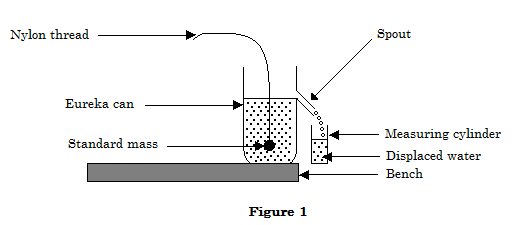
\includegraphics[width=13cm]{./img/2012-1-alt.png}
\end{center}

\item[(b)] Hold a suitable measuring cylinder under the spout and immerse a standard mass of 50 g into eureka can as shown in Figure 1. Water will pass through the spout and will be collected by the measuring cylinder. Wait for it to drop until it starts to cease and take long interval to drop. Record the reading of the water collected.
\item[(c)] Repeat the procedures in 1 (b) for standard masses of 100 g, 150 g, 200 g and 250 g.
\item[(d)] Tabulate your results showing the quantities as follows:\\

\begin{tabular}{|p{4cm}|p{4cm}|p{4cm}|}\hline
Mass (g) & Volume (cm$^3$) & Mass $\div$ Volume (g/cm$^3$) \\ \hline
50 & & \\ \hline
100 & & \\ \hline
150 & & \\ \hline
200 & & \\ \hline
250 & & \\ \hline
\end{tabular}\\[10pt]

\item[(e)] Plot a graph of mass against volume.
\item[(f)] State the nature of the graph.
\item[(g)] From the graph:
\begin{enumerate}
\item[(i)] Calculate the slope.
\item[(ii)] What does the slope of the graph show?
\item[(iii)] What is the relationship between mass and volume?
\item[(iv)] Establish the formula governing the experiment.
\end{enumerate}
\item[(h)] Identify with reasons the best to the least satisfactory method of finding the constant value of mass divide by volume.
\item[(i)] State two possible errors in this experiment.
\item[(j)] How can you minimize errors in 1 (i)?
\end{enumerate}

\pagebreak

\item[2.] You are provided with two plane mirrors, an optical pin, a sheet of plane drawing paper, mirror holder or office pins, a protractor, a ruler and a drawing table. Proceed as follows:
\begin{enumerate}
\item[(a)] Draw two lines at right angles.
\item[(b)] Place the two plane mirrors along the top two lines using the mirror holders or office pins as shown in Figure 2.

\begin{center}
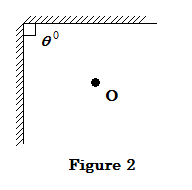
\includegraphics[width=5cm]{./img/2012-2-alt.png}
\end{center}

\item[(c)] Put an optical pin at O when $\theta = 90^\circ$. Look onto one of the mirrors and count the number of images, $n$, you see.
\item[(d)] Repeat the procedures in 2 (c) for $\theta = 72^\circ$, $\theta = 60^\circ$, $\theta = 45^\circ$ and $\theta = 30^\circ$.
\item[(e)] Tabulate your results for the values of $\theta$, $n$ and $\cfrac{360^\circ}{\theta}$.
\item[(f)] Plot a graph of number of images, $n$, against $\cfrac{360^\circ}{\theta}$.
\item[(g)] From the graph:
\begin{enumerate}
\item[(i)] Determine the slope.
\item[(ii)] Find the number of images when $\cfrac{360^\circ}{\theta} = 9$
\item[(iii)] Find the value of the $y$-intercept.
\item[(iv)] Derive the equation relating the number of images and $\cfrac{360^\circ}{\theta}$
\end{enumerate}
\item[(h)] From your experiment:
\begin{enumerate}
\item[(i)] What happens to the number of images as the value angle $\theta$ is reduced?
\item[(ii)] What happens to the number of images when $\theta = 0^\circ$?
\end{enumerate}
\item[(i)] State a possible source of error and how you can minimize it.
\item[(j)] What is the aim of this experiment?
\end{enumerate}
\end{enumerate}
\pagebreak
\index{Past Papers!Physics!2011}
\subsection{2011 - PHYSICS 2A ACTUAL PRACTICAL A}

\begin{enumerate}
\item The aim of this experiment is to determine the mass of a given dry cell size ``AA''. Proceed as follows:
\begin{itemize}
\item[(a)] Locate and note the centre of gravity $C$ of the metre rule by balancing it on the knife edge.
\item[(b)] Suspend the 50 g mass at length `$a$' cm on one side of the metre rule and the 20 g mass together with the dry cell at length `$b$' cm on the other side of the metre rule. Fix the 50 g mass at length 30 cm from the fulcrum and adjust the position of the 20 g mass together with the dry cell until the metre rule balances horizontally. Read and record the values of $a$ and $b$ as $a_0$ and $b_0$ respectively.
\item[(c)] Draw the diagram for this experiment.
\item[(d)] By fixing $a = 5$ cm from fulcrum $C$, find its corresponding length $b$.
\item[(e)] Repeat the procedure in (d) above for $a = 10$ cm, 15 cm, 20 cm and 25 cm. Tabulate your results.
\item[(f)] Draw a graph of `$a$' against `$b$' and calculate its slope $G$.
\item[(g)] Calculate $X$ from the equation $50 = \cfrac{b_0}{a_0}(20 + X)$.
\item[(h)] Comment on the value of $\cfrac{b_0}{a_0}$.
\item[(i)] Sate the principle governing this experiment.
\end{itemize}
\end{enumerate}

\flushright \textbf{(25 marks)}
\begin{enumerate}
\item[2.] You are provided with an ammeter, A, resistance box, R, dry cell, D, a key, K and connecting wires. Proceed as follows:
\begin{enumerate}
\item[(a)] Connect the circuit in series.
\item[(b)] Put $R$ = 1 $\Omega$ and quickly read the value of current $I$ on the ammeter.
\item[(c)] Repeat procedure (b) above for $R$ = 2 $\Omega$, 3 $\Omega$, 4 $\Omega$ and 5 $\Omega$. Record your results in a tabular form.
\item[(d)] Draw the circuit diagram for this experiment.
\item[(e)] Plot the graph of $R$ against $\cfrac{1}{I}$.
\item[(f)] Determine the slope of the graph.
\item[(g)] If the graph obeys the equation $R=\cfrac{E}{I}-r$, then
\begin{enumerate}
\item[(i)] suggest how $E$ and $r$ may be evaluated from your graph.
\item[(ii)] compute $E$.
\item[(iii)] compute $r$.
\end{enumerate}
\item[(h)] State one source of error and suggest one way of minimizing it.
\item[(i)] Suggest the aim of this experiment.
\end{enumerate}

\end{enumerate}

\flushright \textbf{(25 marks)}
\flushleft
\pagebreak
\index{Past Papers!Physics!2010}
\section{2010 - PHYSICS 2A ALTERNATIVE A PRACTICAL}

\begin{enumerate}
\item[1.] The aim of this experiment is to find the mass of the unknown load labeled ``$W$'' and the spring constant $K$. Proceed as follows:

\begin{center}
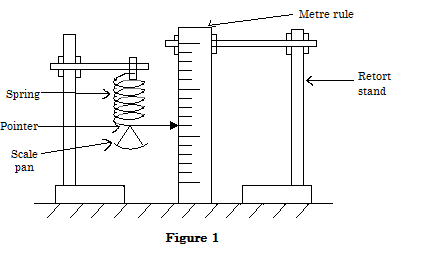
\includegraphics[width=14cm]{./img/2010-1-alt.png}
\end{center}

Set up the apparatus as shown in Figure 1. Put a mass of 50 g on the scale pan and record the equilibrium position $X_0$ of the pointer. Put on the scale pan the unknown weight marked $W$. Without removing $W$ and the 50 g mass in the scale pan, add a load $L$ of 50 g and record the new position of the pointer $X$. Calculate the extension $E = (X - X_0)$. Repeat this process for $L$ = 100 g, 150 g, 200 g and 250 g.
\begin{enumerate}
\item[(a)] Record you conclusions as shown in Table 1.\\[10pt]

Equilibrium position $X_0$..................\\[10pt]

Table 1\\[10pt]

%\begin{center}
\begin{tabular}{|p{3cm}|p{3cm}|p{3cm}|} \hline
\multicolumn{1}{|c|}{Load (g)} & \multicolumn{1}{c|}{$X$ (cm)} & \multicolumn{1}{c|}{$E = X - X_0$ (cm)} \\ \hline
\multicolumn{1}{|c|}{50} & & \\ \hline
\multicolumn{1}{|c|}{100} & & \\ \hline
\multicolumn{1}{|c|}{150} & & \\ \hline
\multicolumn{1}{|c|}{200} & & \\ \hline
\multicolumn{1}{|c|}{250} & & \\ \hline
\end{tabular}\\[10pt]
%\end{center}

\item[(b)] Plot the graph of load L against absolute value of extension E. The scale of the vertical axis should be chosen to range from 200 g to 300 g.
\item[(c)] From the graph, determine the unknown weight marked W, given that L = KE + W where K is a constant.
\item[(d)] What does the gradient of the graph represent?
\item[(e)] State the sources of errors and precautions that should be taken in the experiment.
\end{enumerate}
\end{enumerate}
\flushright \textbf{(25 marks)}

\pagebreak

\begin{enumerate}
\item[2.] The aim of this experiment is to determine the refractive index of water. Proceed as follows:

\begin{center}
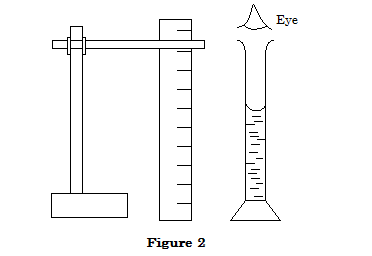
\includegraphics[width=10cm]{./img/2010-2-alt.png}
\end{center}

\begin{enumerate}
\item[(a)] Arrange your apparatus as in Figure 2. Put about 150 cm$^3$ of clear water in the measuring cylinder. Drop an office pin at the bottom so that it rests touching the wall of the cylinder.
\item[(b)] Look in the cylinder from Figure 2. Use another office pin as a search pin, move it up and down outside the cylinder, and locate the image position by no parallax method. Locate the image position of the ruler. Measure and record the depth ($H_1$) of the image. Measure and record the depth ($H_2$) of water. Repeat the experiment with 175 cm$^3$, 200 cm$^3$, 225 cm$^3$ and 250 cm$^3$ of water in the measuring cylinder.
\item[(c)] 
\begin{enumerate}
\item[(i)] Record in Table 2 your values of $H_1$ and $H_2$ corresponding to the volumes of water in the measuring cylinder.\\[10pt]

Table 2\\[10pt]

%\begin{center}
\begin{tabular}{|p{3cm}|p{3cm}|p{3cm}|} \hline
\multicolumn{1}{|c|}{Volume of water V (cm)} & \multicolumn{1}{c|}{$H_1$} & \multicolumn{1}{c|}{$H_2$} \\ \hline
\multicolumn{1}{|c|}{150} & & \\ \hline
\multicolumn{1}{|c|}{175} & & \\ \hline
\multicolumn{1}{|c|}{200} & & \\ \hline
\multicolumn{1}{|c|}{225} & & \\ \hline
\multicolumn{1}{|c|}{250} & & \\ \hline
\end{tabular}\\[10pt]
%\end{center}

\item[(ii)] Plot the graph of $H_2$ versus $H_1$.
\item[(iii)] Determine the slope of the graph.
\item[(iv)] What is the physical meaning of the slope?
\item[(v)] State sources of error in this experiment.
\end{enumerate}
\end{enumerate}
\end{enumerate}
\flushright \textbf{(25 marks)}

\pagebreak

\begin{enumerate}
\item[3.] The aim of this experiment is to determine the resistivity of an electrical conductor $P$.

\begin{center}
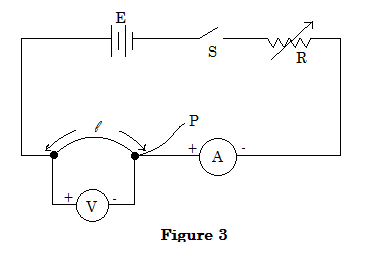
\includegraphics[width=10cm]{./img/2010-3-alt.png}
\end{center}

With $P$ having a length $l = 50$ cm, connect up the circuit as shown in Figure 3. Close one key S and adjust the rheostat R so that the current in $P$ is 0.20 A. Record the current $I$ and the potential difference $V$ between its ends.\\[10pt]

Repeat the procedure with current $I = $0.30 A, 0.40 A, 0.50 A and 0.60 A.
\begin{enumerate}
\item[(a)] Record your results in Table 3.\\[10pt]

Table 3\\[10pt]

%\begin{center}
\begin{tabular}{|p{3cm}|p{3cm}|} \hline
\multicolumn{1}{|c|}{Current $I$ (A)} & \multicolumn{1}{c|}{P.d. (volts)} \\ \hline
\multicolumn{1}{|c|}{0.20} &  \\ \hline
\multicolumn{1}{|c|}{0.30} &  \\ \hline
\multicolumn{1}{|c|}{0.40} &  \\ \hline
\multicolumn{1}{|c|}{0.50} &  \\ \hline
\multicolumn{1}{|c|}{0.60} &  \\ \hline
\end{tabular}\\[10pt]
%\end{center}

\item[(b)] Plot a graph of $V$ against $I$ and calculate the slope $G$.
\item[(c)] Deduce the resistivity of the conductor $P$ given that; $\rho = \cfrac{G\pi d^2}{4l}$.\\[10pt]
Where $\rho$ = resistivity\\
$d$ = diameter of $P$ (measured using the micrometer screw gauge provided).
\end{enumerate}
\end{enumerate}

\flushright \textbf{(25 marks)}
\flushleft
\pagebreak
\index{Past Papers!Physics!2009}
\subsection{2009 - PHYSICS 2A ALTERNATIVE A PRACTICAL}

\begin{enumerate}
\item[1.] In this experiment you are required to find the relationship between the length of a simple pendulum and its period. Proceed as follows:
\begin{itemize}
\item[(a)] Suspend a simple pendulum of length L = 100 cm. Displace the pendulum through a small angle so that it swings parallel to the edge of the bench or table, determine the time for 20 oscillations. Continue reducing the length of the pendulum by 10 cm each time and obtain a total of six readings.
\item[(b)] Record your readings in a table as shown below.


\begin{tabular}{|p{2.5cm}|p{2.5cm}|p{2.5cm}|p{2.5cm}|p{2.5cm}|} \hline
Length of pendulum L (cm) & Log$_{10}$L & Time for 20 oscillations & Period T & Log$_{10}$T \\ \hline
&&&& \\ 
&&&& \\ 
&&&& \\ 
&&&& \\ 
&&&& \\ 
&&&& \\ 
&&&& \\ 
&&&& \\ \hline
\end{tabular}\\[10pt]

\noindent Assuming that T $ \propto $ L$^a$, we have T = $k$L$^a$ and taking logarithms to base ten on both sides we get $\log_{10}$T = $a\log_{10}$L + $\log_{10}k$.

\begin{itemize}
\item[(i)] Plot a graph of $\log_{10}$T (vertical axis) against $\log_{10}$L (horizontal axis) hence determine the values of $a$ and $k$ each correct to one decimal place.
\item[(ii)] From your answer in (i) above write down the values of $a$ and $k$ each in the form of $\cfrac{b}{c}$ where $b$ and $c$ are integers (i.e. whole numbers).
\item[(iii)] From the assumption and your answer in (ii) deduce the form of the equation governing the motion of the simple pendulum.
\end{itemize}

\end{itemize}
\end{enumerate}
\flushright \textbf{(25 marks)}


\begin{enumerate}
\item[2.] The aim of this experiment is to determine the refractive index $\eta$ of a given glass block.

\begin{center}
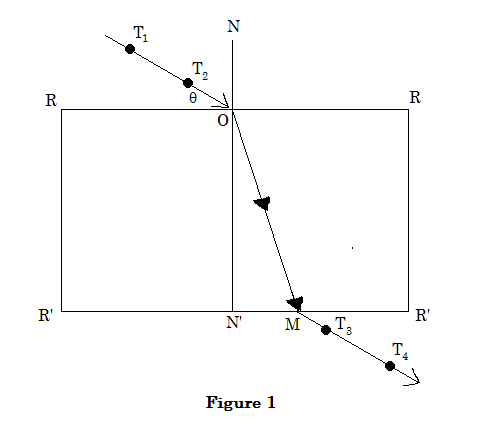
\includegraphics[width=8cm]{./img/2009-2-alt.png}
\end{center}

Place the rectangular glass block on the white paper on a drawing board. Using a pencil trace the outline of the block. Remove the glass block and draw a normal NOM near the left end of the block (Figure 1).\\[10pt]

\noindent Using a protractor and a pencil measure $\theta = 20^\circ$, draw a line making the angle $20^\circ$ with the surface RR of the block. Erect two pins T$_1$ and T$_2$ on this line and at a suitable distance from one another. Return the block and erect the pins T$_3$ and T$_4$ at positions such that they lie in a straight line with pins T$_1$ and T$_2$ as seen through the block. Now remove the block and draw a complete path of the ray (Figure 1).\\[10pt]

\noindent Measure the length MN$'$ and ON$'$: Repeat the procedure for values of $\theta = 30^\circ, 40^\circ$ and $60^\circ$ respectively. In each case make a drawing on a fresh part of the drawing paper.

\begin{itemize}
\item[(a)] Record the values of $\theta$, MN$'$, ON$'$, $\cfrac{\text{MN}'}{\text{ON}'}$ and $\cos \theta$ in a tabular form.
\item[(b)] Plot a graph of $\cfrac{\text{MN}'}{\text{ON}'}$ against $\cos \theta$.
\item[(c)] Find the slope $G$ of the graph.
\item[(d)] Calculate the value of the refractive index $\eta$; given that $G = \cfrac{1}{\eta}$.
\item[(e)] State two sources of errors. \hfill \textbf{(25 marks)}
\end{itemize}

\end{enumerate}


\begin{enumerate}
\item[3.] The aim of this experiment is to verify Ohm's Law.

\begin{center}
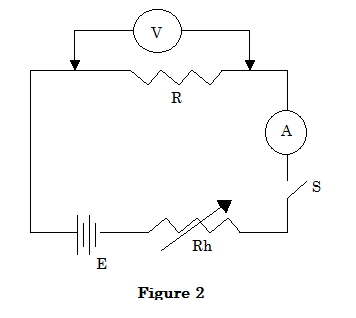
\includegraphics[width=7cm]{./img/2009-3-alt.png}
\end{center}

\begin{itemize}
\item[(a)] Set up the apparatus as shown on Figure 2, close switch S. Adjust the Rheostat Rh by sliding slowly from one end, read and record the value V of the voltmeter and current I of the ammeter.
\item[(b)] Repeat the experiment by changing the Rheostat slider to obtain about five pair of readings.\\[10pt]

\textbf{NB:} Adjust the Rheostat until when the pointer is exactly on the division of the metre scale.\\[10pt]

Table of results\\[10pt]
\begin{tabular}{|c|c|c|c|c|c|c|c|}\hline
V (V)&&&&&&&\\ \hline
I (A)&&&&&&& \\ \hline
\end{tabular}

\item[(c)] Plot a graph of V (vertical axis) against I (horizontal axis).
\item[(d)] 
\begin{itemize}
\item[(i)] Find the slope of the graph.
\item[(ii)] What is the relation between V and I?
\item[(iii)] Find the resistance R. \hfill \textbf{(25 marks)}
\end{itemize}
\end{itemize}

\end{enumerate}
\flushleft

\pagebreak
\index{Past Papers!Physics!2008}
\section{2008 - PHYSICS 2A  ALTERNATIVE A PRACTICAL}

\begin{enumerate}
\item[1.] The aim of this experiment is to investigate whether string A obeys Hooke's law.

\begin{center}
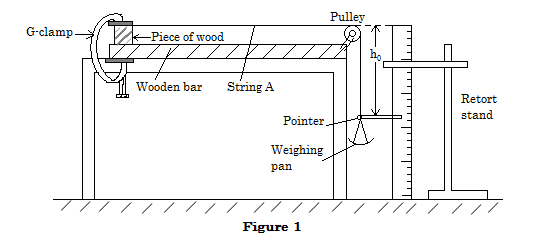
\includegraphics[width=15cm]{./img/2008-1-alt.png}
\end{center}

Proceed as follows:\\[6pt]

Clamp string A at one end, attach a weighing pan at the other end and a pointer to give a reading on a scale as shown in figure 1 above.\\[6pt]

Measure the height, $h_0$ when the pan is empty.\\[6pt]

Place 50 g mass on the pan and record the new height $h$ indicated by the pointer.\\[6pt]

Add another 50 g mass each time up to 300 g, and record the corresponding values of $h$ for added mass.

\begin{enumerate}
\item[(a)] Tabulate your results as shown in the table below.
\item[] $h_0 = $ \begin{tabular}{p{1.5cm}}
\\ \hline
\end{tabular} cm.\\[10pt]

\begin{tabular}{|c|c|c|c|c} \hline
Mass, $m$ (g) & Height, $h$ (cm) & Extension ($h - h_0$) & Stretching \\
&&(cm)&force, $F$ (N) \\ \hline
50&&& \\ 
100&&& \\ 
150&&& \\ 
200&&& \\ 
250&&& \\ 
300&&& \\ \hline
\end{tabular}\\[10pt]
\item[(b)] Plot a graph of force $F$ (N) against extension (cm).
\item[(c)] From the graph find the
\begin{enumerate}
\item[(i)] slope, K of the graph.
\item[(ii)] extension caused by a mass of 180 g.
\end{enumerate}
\item[(d)] Deduce whether string A obeys Hooke's law.
\item[(e)] State the law. \hfill \textbf{(25 marks)}
\end{enumerate}
\end{enumerate}

\begin{enumerate}
\item[2.] You are provided with a glass block, four sheets of drawing paper, four optical pins (or office pins) and a drawing board.\\[6pt]

Proceed as follows:\\[6pt]

Place the glass block flat on the drawing paper fixed to the drawing board and with a sharp pencil, draw its outline.

\begin{center}
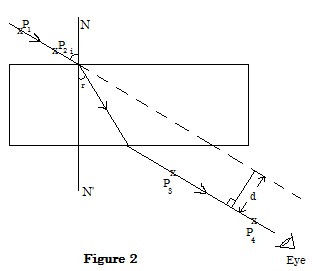
\includegraphics[width=9cm]{./img/2008-2-alt.png}
\end{center}

Remove the glass block and draw a normal NN' to the longer edge of the block (see fig. 2).\\
Draw a line making an angle of incidence ($i$) of 30$^\circ$. Stick two vertical pins P$_1$ and P$_2$ on this line. Replace the glass block. Stick two more pins P$_3$ and P$_4$ on the other side of the block so that they appear to be in the same straight line with the images of pins P$_1$ and P$_2$ as seen through the block.\\
Remove the block and draw the complete path of the ray entering and leaving the block.\\
Measure the angle of refraction ($r$).\\[6pt]

Produce the incident ray as shown in fig. 2 and measure the perpendicular distance ($d$) between the incident ray and the emergent ray.\\
Repeat this procedure for angles of incidence of $40^\circ$, $50^\circ$, $60^\circ$ and $70^\circ$. In each case draw the block again on a fresh part of the paper.
\begin{enumerate}
\item[(a)] Record your results in a table as follows:
\begin{tabular}{|p{0.15\textwidth}|p{0.15\textwidth}|p{0.15\textwidth}|p{0.15\textwidth}|p{0.15\textwidth}|} \hline
\multicolumn{1}{|c|}{$i^\circ$} & \multicolumn{1}{c|}{$r^\circ$} & \multicolumn{1}{c|}{$d$ (cm)} & \multicolumn{1}{c|}{$d\cos{r}$ (cm)} & \multicolumn{1}{c|}{$\sin{(i-r)}$} \\ \hline
\multicolumn{1}{|c|}{30}&&&& \\
\multicolumn{1}{|c|}{40}&&&& \\
\multicolumn{1}{|c|}{50}&&&& \\
\multicolumn{1}{|c|}{60}&&&& \\
\multicolumn{1}{|c|}{70}&&&& \\ \hline
\end{tabular}\\[10pt]
\item[(b)] Plot a graph of $d \cos{r}$ (vertical axis) against $\sin{(i - r)}$ (horizontal axis).
\item[(c)] Find the gradient of the graph.
\item[(d)] Measure the width of the glass block.
\item[(e)] How is the gradient related to the with of the glass block?
\item[] NB: Hand in your diagrams together with your answer booklet. \hfill \textbf{(25 marks)}
\end{enumerate}
\end{enumerate}

\begin{enumerate}
\item[3.] The aim of this experiment is to determine the resistance of a wire W.\\
Proceed as follows:
\begin{enumerate}
\item[(a)] Connect in series the full length of wire W of unknown resistance, battery B (3 V), a switch K, a rheostat Rh of a few ohms and an ammeter A of $0 - 1$ A.\\
Connect the voltmeter V of $0 - 3$ V across W. Check that the +ve side of the ammeter A and the +ve side of the voltmeter V are both on the +ve side of the battery B.
\item[(b)] Switch on the current. Adjust the rheostat to obtain five widely different values of $V$ and corresponding values of current $I$.
\item[(c)] Tabulate your results as follows:\\[10pt]
\begin{tabular}{|p{4cm}|p{4cm}|} \hline
\multicolumn{1}{|c|}{Potential difference} & \multicolumn{1}{c|}{Current $I$ (amperes)} \\
\multicolumn{1}{|c|}{$V$ (volts)} & \\ \hline
& \\ 
& \\ 
& \\ \hline
\end{tabular}
\item[(d)]
\begin{enumerate}
\item[(i)] Draw a circuit diagram.
\item[(ii)] Plot a graph of potential difference $V$ against current $I$.
\item[(iii)] Find the slope of the graph.
\item[(iv)] Determine the resistance of the wire W.
\item[(v)] Mention \textbf{two (2)} main precautions to be taken in this experiment.
\end{enumerate}
\end{enumerate}
\end{enumerate}
\flushright \textbf{(25 marks)}
\flushleft
\pagebreak
\index{Past Papers!Physics!2007}
\section{2007 - PHYSICS 2A ALTERNATIVE A PRACTICAL}

\begin{enumerate}
\item[1.] The aim of this experiment is to determine the mass of a given object ``B'', and the constant of the spring provided.

\begin{center}
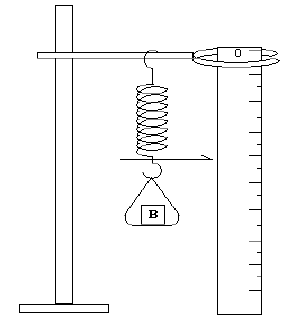
\includegraphics[width=7cm]{./img/2007-1-alt.png}
\end{center}

\begin{itemize}
\item[]
\begin{itemize}
\item[(i)] Set up the apparatus as shown in Fig. 1 with zero mark of the metre-rule at the top of the rule and record the scale reading by the pointer, $S_0$.
\item[(ii)] Place the object ``B'' and standard weight (mass) W equal to 20 g in the pan and record the new pointer reading $S_1$. Calculate the extension, $e = S_1 - S_0$ in cm.
\item[(iii)] Repeat the procedure in (ii) above with W = 40 g, 60 g, 80 g and 100 g.
\end{itemize}
\item[(a)] Record your results in tabular form as shown below:\\
Table of Results:

\begin{tabular}{|p{2cm}|p{3cm}|p{3cm}|p{3cm}|}\cline{1-1}
\multicolumn{1}{|p{2cm}|}{$S_0 = $}&\multicolumn{2}{c}{} & \multicolumn{1}{p{2.5cm}}{} \\ \hline
\multicolumn{1}{|c|}{Mass} & \multicolumn{1}{c|}{Force, F (N)} & \multicolumn{1}{c|}{Pointer reading $S_1$} & \multicolumn{1}{c|}{Extension}\\
\multicolumn{1}{|c|}{(kg)} & \multicolumn{1}{c|}{} & \multicolumn{1}{c|}{(cm)} & \multicolumn{1}{c|}{$= S_1 - S_0$ (cm)}\\ \hline
\multicolumn{1}{|c|}{0} & \multicolumn{1}{c|}{} & \multicolumn{1}{c|}{} & \multicolumn{1}{c|}{}\\ 
\multicolumn{1}{|c|}{0.02} & \multicolumn{1}{c|}{} & \multicolumn{1}{c|}{} & \multicolumn{1}{c|}{}\\ 
\multicolumn{1}{|c|}{0.04} & \multicolumn{1}{c|}{} & \multicolumn{1}{c|}{} & \multicolumn{1}{c|}{}\\ 
\multicolumn{1}{|c|}{0.06} & \multicolumn{1}{c|}{} & \multicolumn{1}{c|}{} & \multicolumn{1}{c|}{}\\ 
\multicolumn{1}{|c|}{0.08} & \multicolumn{1}{c|}{} & \multicolumn{1}{c|}{} & \multicolumn{1}{c|}{}\\ 
\multicolumn{1}{|c|}{0.10} & \multicolumn{1}{c|}{} & \multicolumn{1}{c|}{} & \multicolumn{1}{c|}{}\\ \hline
\end{tabular}
\item[(b)] Plot graph of Force F (vertical axis) against extension $e$ (horizontal axis).
\item[(c)] Use your graph to evaluate
\begin{itemize}
\item[(i)] mass of B
\item[(ii)] spring constant, K, given that force, extension, constant and weight of B are related as follows:\\
F = K$e$ - B
\end{itemize}
\end{itemize}

\end{enumerate}
\flushright \textbf{(25 marks)}



\begin{enumerate}
\item[2.] The aim of this experiment is to find the refractive index of a glass block. Proceed as following:\\[10pt]

Place the given glass block in the middle of the drawing paper on the drawing board. Draw lines along the upper and lower edge of the glass block. Remove the glass block and extend the line you have drawn. Represent the ends of those line segments as SS$^1$ and TT$^1$. Draw the normal NN$^1$ to the parallel lines SS$^1$ and TT$^1$ as shown in Fig. 2(a).

\begin{center}
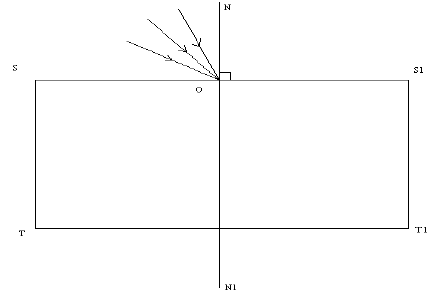
\includegraphics[width=8cm]{./img/2007-2a-alt.png}
\end{center}

Draw five evenly spaced lines from O to represent incident rays at different angles of incidence (10$^\circ$, 20$^\circ$, 30$^\circ$, 40$^\circ$ and 50$^\circ$ from the normal). Replace the glass block carefully between SS$^1$ and TT$^1$. Stick two pins P$_1$ and P$_2$ as shown in Fig. 2(b) as far apart as possible along one of the lines drawn to represent an incident ray. Locate an emergent ray by looking through the block and stick pins P$_3$ and P$_4$ exactly in line with images I$_1$ and I$_2$ of pins P$_1$ and P$_2$. Draw the emergent ray and repeat the procedure for all the incident rays you have drawn. Finally draw in the corresponding refracted rays.\\[10pt]

NOTE: The drawing paper should be handed in together with other answer sheets.

\begin{center}
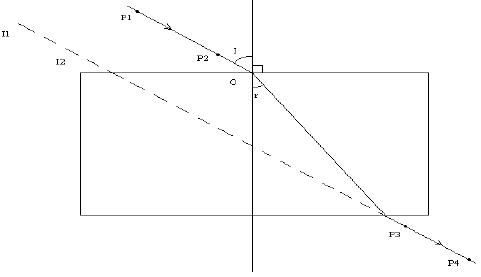
\includegraphics[width=10cm]{./img/2007-2b-alt.png}
\end{center}

\begin{itemize}
\item[(a)] Record the angles of incidence I and the measured corresponding angles of refraction ``r'' in a table. Your table of results should include the values of $\sin$ I and $\sin$ r.
\item[(b)] Plot the graph of $\sin$ I (vertical - axis) against $\sin$ r (horizontal - axis).
\item[(c)] Determine the slope of the graph.
\item[(d)] What is the refractive index of the glass block used?
\item[(e)] Mention any sources of errors in this experiment.
\end{itemize}

\end{enumerate}
\flushright \textbf{(25 marks)}


\begin{enumerate}
\item[3.] The aim of this experiment is to determine the potential fall along a uniform resistance wire carrying a steady current.\\[10pt]

Proceed as follows:

\begin{center}
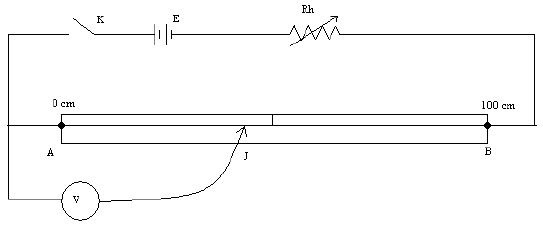
\includegraphics[width=12cm]{./img/2007-3-alt.png}
\end{center}

Connect up the circuit as shown in Fig. 3. Adjust the rheostat so that when the sliding contact J is near B, and the key is closed the voltmeter V indicates an almost full scale deflection. Do not alter the rheostat again.\\

Close key K and make contact with J, so that AJ = 10 cm. Record the potential different V volts between A and J as registered on the voltmeter.\\

Repeat this procedure for AJ = 20 cm, 30 cm, 50 cm and 70 cm.

\begin{itemize}
\item[(a)] Tabulate your results for the values of AJ and V.
\item[(b)] Plot a graph of V (vertical axis) against AJ (horizontal axis).
\item[(c)] Calculate the slope of the graph.
\item[(d)] What is your comment on the slope?
\item[(e)] State any precautions on the experiment.
\end{itemize}

\end{enumerate}
\flushright \textbf{(25 marks)}
\flushleft
\pagebreak
\index{Past Papers!Physics!2006}
\section{2006 - PHYSICS 2A ALTERNATIVE A PRACTICAL}

\begin{enumerate}
\item[1.] In this experiment you are required to determine the mass of unknown object ``X''.

\begin{center}
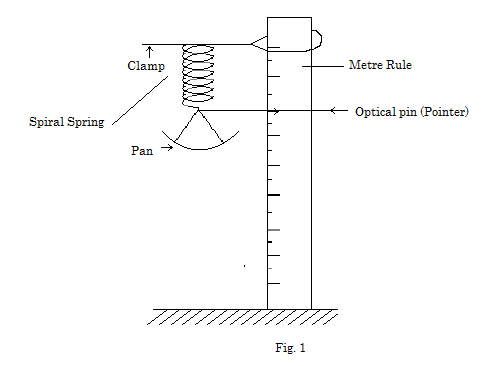
\includegraphics[width=10cm]{./img/2006-1-alt.png}
\end{center}

Assemble the pieces of apparatus as shown in Figure 1, with zero mark scale of the rule at the lower most end.\\

Record the reading of the position of pointer on the scale of metre-rule when the pan is empty as $S_0$.\\

Put 20 g to the pan and record pointer reading $S$.\\

Find extension $e = S - S_0$ cm.\\

Repeat the procedure for mass of 40 g, 60 g, 80 g and 100 g. Put object X on the pan and record its pointer reading.

\begin{itemize}
\item[(a)] Summarize your results in a table as follows:\\[10pt]
\begin{center}
\begin{tabular}{|l|c|c|c|c|c|c|} \hline
Mass on pan (g) &20&40&60&80&100&X \\ \hline
Pointer reading (cm) &&&&&& \\ \hline
Extension, $e = S - S_0$ (cm) &&&&&& \\ \hline
\end{tabular} \\[10pt]
\end{center}
\item[(b)] Plot graph of mas against extension (m Vs. $e$).
\item[(c)] Find slope, P, of your graph.
\item[(d)] Find mass X.
\item[(e)] Find Q, given that Q = P $\times$ $e_\text{x}$, where $e_\text{x}$ is extension of X.
\item[(f)] Comment on Q and X.
\end{itemize}


\end{enumerate}

\begin{enumerate}
\item[2.] Set up the experiment as shown in the diagram below using plane mirror, soft board, three pins and a white sheet of paper.

\begin{center}
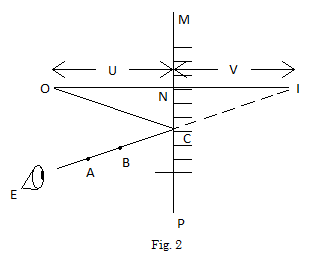
\includegraphics[width=6cm]{./img/2006-2-alt.png}
\end{center}

Fix a white sheet of paper on the soft board. Draw a line across the width at about the middle of the white sheep (MP). Draw line ONI perpendicular to MP.\\

Fix optical pin O to make ON = U = 3 cm. By using plasticine or otherwise, fix plane mirror along portion of MP with O in front of the mirror. With convenient position of eye, E, look into the mirror and fix optical pins A and B to be in line with image, I, of pin O.\\

Measure and record NI = V. Repeat procedure for U = 6 cm, 9 cm and 12 cm.

\begin{itemize}
\item[(a)] Tabulate your results as follows:\\[10pt]

\quad \quad \begin{tabular}{|l|c|c|c|c|} \hline
U (cm) &3&6&9&12 \\ \hline
V (cm) &&&& \\ \hline
\end{tabular} \\[10pt]

\item[(b)] Plot graph of U against V.
\item[(c)] Calculate slope, m, of the graph to the nearest whole number.
\item[(d)] State relationship between U and V.
\item[(e)] Write equation connecting U and V using numerical value of m with symbols U and V.
\item[(f)] From your equation give position of the image when object is touching the face of the mirror.
\end{itemize}

\end{enumerate}


\begin{enumerate}
\item[3.] You are required to determine the unknown resistance labeled X using a metre bridge circuit. Connect your circuit as shown below, where R is a resistance box, G is a galvanometer, J is a jockey and others are common circuit components.

\begin{center}
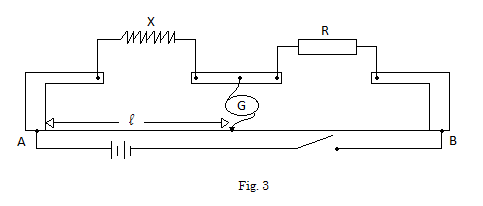
\includegraphics[width=14cm]{./img/2006-3-alt.png}
\end{center}

Procedure:\\

With R = 1 $\Omega$, obtain a balance point on a metre bridge wire AB using a jockey J. Note the length $l$ in centimetres. Repeat the experiment with R equal to 2 $\Omega$, 4 $\Omega$, 7 $\Omega$ and 10 $\Omega$.\\

Tabulate your results for R, $l$ and $^1/_l$.

\begin{itemize}
\item[(a)]
\begin{itemize}
\item[(i)] Plot a graph of R (vertical axis) against $^1/_l$ (horizontal axis).
\item[(ii)] Determine the slope S of your graph.
\item[(iii)] Using your graph, find the value of R for which $^1/_l = 0.02$.
\end{itemize}
\item[(b)] Read and record the intercept R$_0$ on the vertical axis.
\item[(c)] Given that,\\
\quad \quad R = $\cfrac{100\text{X}}{l}$ - X\\
Use the equation and your graph to determine the value of X.
\item[(d)] Comment on your results in (a)(iii), (b) and (c) above.
\end{itemize}

\end{enumerate}
\pagebreak
\index{Past Papers!Physics!2005}
\subsection{2005 - PHYSICS 2A ALTERNATIVE A PRACTICAL}

\begin{enumerate}
\item[1.] The aim of this experiment is to determine the mass of unknown weight labelled \textbf{X} and the force constant of the spring \textbf{k}.

\begin{center}
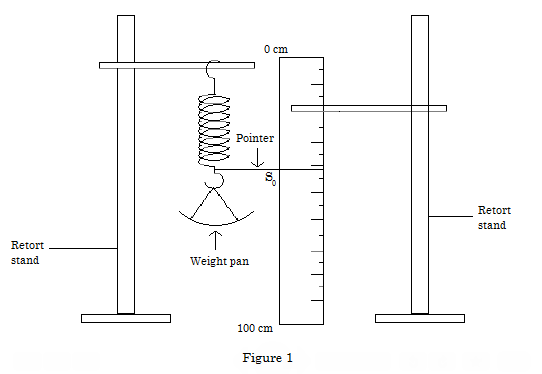
\includegraphics[width=12cm]{./img/2005-1-alt.png}
\end{center}

Set up the apparatus provided as shown in figure 1 above. Add 50 g mass on to the weight pan so that any ``kinks'' in the spring are removed. Leave this weight for the whole experiment but ignore it in all readings. Record the scale reading $S_0$. Add 50 g on to the weight pan and record the new scale reading $S$. Calculate the extension ($e = S - S_0$) caused by the weight. Repeat with different weights ($W$) to obtain at least five readings. Tabulate your results. Replace the weights ($W$) by the weight \textbf{X} provided and find the corresponding extension.\\[10pt]

Record this extension as $S_{\text{X}}$ ............. cm

\begin{enumerate}
\item[(a)] Plot a graph of load against extension.
\item[(b)]
\begin{enumerate}
\item[(i)] Find the gradient (G) of your graph.
\item[(ii)] What is the physical meaning of the gradient?
\end{enumerate}
\item[(c)] From the graph, what is the mass of the weight labelled \textbf{X}?
\end{enumerate}

\item[2.] The aim of this experiment is to find the critical angle \textbf{C} of the given glass block.

\begin{center}
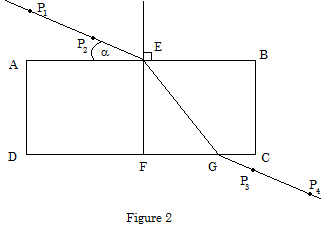
\includegraphics[width=10cm]{./img/2005-2-alt.png}
\end{center}

\textbf{Proceed as follows:}\\[10pt]

Place a white sheet of paper on the drawing board. Place the glass block, with one of its largest surfaces top most on top of the white paper. Mark the outline of the glass block on the paper with a pencil. Then remove the glass block and draw a line which cuts its largest sides normally at E and F as shown in figure 2 above. \\[10pt]

Using a protractor draw an angle $\alpha = 30^\circ$ with the glass block. Replace the glass block in its original position and stick the first pin P$_1$ and second pin P$_2$ along the line of angle $\alpha = 30^\circ$. Stick the third and fourth pins P$_3$ and P$_4$ respectively on the opposite side of the glass block such that P$_3$ and P$_4$ fall on a straight line with P$_1$ and P$_2$ when viewed through side CD of the glass block. \\[10pt]

Remove the glass block and trace the straight path taken by the ray G P$_3$ P$_4$. Using a ruler, join G and E. \\[10pt]

Measure the angle of refraction $r^\circ$, then calculate the values of $\cos{\alpha}$ and $\sin{r^\circ}$. Repeat the same procedure for values $\alpha = 40^\circ$, $50^\circ$, $60^\circ$, $70^\circ$ and $80^\circ$. Record your results in tabular form for the values of $\alpha$, $r^\circ$, $\sin{r^\circ}$ and $\cos{\alpha}$.

\begin{enumerate}
\item[(a)] Plot a graph of $\sin{r^\circ}$ (vertical axis) against $\cos{\alpha}$ (horizontal axis).
\item[(b)] Find the slope of the graph.
\item[(c)] Calculate the value of $C$ where slope = $\sin{C}$.
\item[(d)] State the possible sources of error and precautions you have taken during the experiment.
\end{enumerate}

\item[3.] The aim of this experiment is to determine the \textbf{e.m.f. E} and internal resistance \textbf{r} of a cell.

\begin{center}
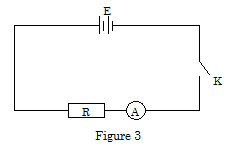
\includegraphics[width=7cm]{./img/2005-3-alt.png}
\end{center}

\begin{enumerate}
\item[(a)] Connect the circuit as shown in figure 3 above. Put $R = 1 \Omega$ and quickly read the value of $i$ on the ammeter.
\item[(b)] Repeat the procedure in 3 (a) above, for values of $R = 2 \Omega$, $3 \Omega$, $4 \Omega$ and $5 \Omega$ respectively.
\item[(c)] Tabulate your results and complete the following table.
\begin{center}
\begin{tabular}{|c|c|c|} \hline
\textbf{Resistance $R$ ($\Omega$)} & \textbf{Current $i$ (A)} & \textbf{$\cfrac{1}{i} \left(\text{A}^{-1}\right)$ } \\ \hline
1&& \\
2&& \\
3&& \\
4&& \\
5&& \\ \hline
\end{tabular} \\[10pt]
\end{center}
\item[(d)] Plot the graph of $R$ against $\cfrac{1}{i}$.
\item[(e)] The graph uses the equation $R = \cfrac{E}{i} - r$.
\begin{enumerate}
\item[(i)] Suggest how $E$ and $r$ may be evaluated from your graph.
\item[(ii)] Evaluate $E$ for one cell.
\item[(iii)] Evaluate $r$ for one cell.
\end{enumerate}
\item[(f)] State one source of error and suggest one way of minimizing it.
\end{enumerate}

\end{enumerate}
\pagebreak
\index{Past Papers!Physics!2004}
\subsection{2004 - PHYSICS 2A ALTERNATIVE A PRACTICAL}

\begin{enumerate}
\item[1.] The aim of this experiment is to determine the mass of a given dry cell, size ``AA''.\\[5pt]

You are provided with a dry cell, a knife edge, two weights 50 g and 20 g, and a metre rule.\\[5pt]

Proceed as follows:
\begin{enumerate}
\item[(a)] Locate and note the centre of gravity C of the metre rule by balancing on the knife edge.
\item[(b)] Suspend the 50 g mass on one side of the metre rule, and 20 g together with the dry cell on the other side of the metre rule adjusting their position until the metre rule balances horizontally, as shown in Figure 1 below.

\begin{center}
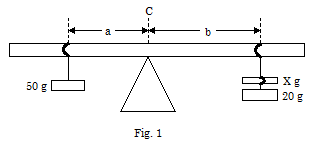
\includegraphics[width=10cm]{./img/2004-1-alt.png}
\end{center}

\item[(c)] By fixing a = 5 cm from C find its corresponding length, b, from C.
\item[(d)] Repeat and tabulate your results using a = 10 cm, 15 cm, 20 cm and 25 cm.
\item[(e)] Draw a graph of ``a'' against ``b'' and calculate its slope G.
\item[(f)] Calculate X from the equation $\text{G} = \cfrac{20 + \text{X}}{50}$. \hfill \textbf{(25 marks)}
\end{enumerate}


\item[2.] You are provided with a glass block, drawing board, optical pins and plane papers.\\

Place a white piece of paper on the drawing board. Place the glass block with one of its largest surface top most on top of the white paper. Mark the outline of the glass block on the paper with a pencil. Remove the glass block and draw a normal as shown in Figure 2 below.

\begin{center}
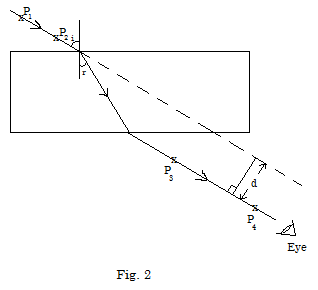
\includegraphics[width=10cm]{./img/2004-2-alt.png}
\end{center}

\begin{enumerate}
\item[(a)] Draw a line making an angle of incidence, $i$ of $30^\circ$. Erect two pins P$_1$ and P$_2$ on this line at a suitable distance apart. Replace the glass block and erect two more pins P$_3$ and P$_4$ at positions which appear to be in a straight line with the other two pins as seen through the glass block from the other side.\\[10pt]

Remove the glass block and draw the complete path of the ray (see Fig. 2). Measure the angle of refraction, $r$.
\item[(b)]
\begin{enumerate}
\item[(i)] Extend the direction of the incident ray as shown by the dotted line.
\item[(ii)] Measure the perpendicular distance `$d$' between extended incident ray and the emergent ray.
\end{enumerate}
\item[(c)] Repeat the procedure in (a) and (b) above for angles of incidence of $30^\circ$, $40^\circ$, $50^\circ$, $60^\circ$ and $70^\circ$. (In each case make your drawings on a fresh part of the drawing paper).
\item[(d)] Tabulate your results as shown in Table 1 below.
\begin{center}
\begin{tabular}{|p{0.15\textwidth}|p{0.15\textwidth}|p{0.15\textwidth}|p{0.15\textwidth}|p{0.15\textwidth}|} \hline
\multicolumn{1}{|c|}{$i$ (deg)} & \multicolumn{1}{c|}{$r$ (deg)} & \multicolumn{1}{c|}{$d$ (cm)} & \multicolumn{1}{c|}{$d\cos{r}$} & \multicolumn{1}{c|}{$\sin{(i-r)}$} \\ \hline
\multicolumn{1}{|c|}{30}&&&& \\
\multicolumn{1}{|c|}{40}&&&& \\
\multicolumn{1}{|c|}{50}&&&& \\
\multicolumn{1}{|c|}{60}&&&& \\
\multicolumn{1}{|c|}{70}&&&& \\ \hline
\end{tabular}\\[10pt]
\end{center}
\begin{enumerate}
\item[(i)] Plot a graph of $d\cos{r}$ against $\sin{(i-r)}$.
\item[(ii)] Find the gradient of the graph.
\item[(iii)] Measure the width of the glass block.
\item[(iv)] How is the gradient of the graph in 2 (a)(ii) and the width of the glass block in 2 (a)(iii) related?\\[5pt]
\end{enumerate}
\item[] NB: \quad Hand in your diagrams (drawings) together with your answer booklet. 
\item[] \flushright \textbf{(25 marks)}

\end{enumerate}

\item[3.] Determine the resistivity $\rho$ of the wire labelled W and the internal resistance of the battery provided.\\

Proceed as follows:

\begin{center}
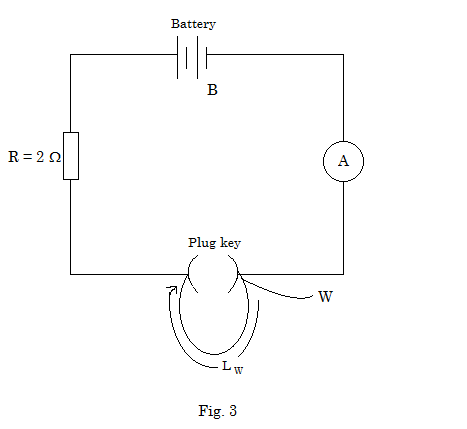
\includegraphics[width=10cm]{./img/2004-3-alt.png}
\end{center}

Connect the circuit as shown in fig. 3 above. With the plug key open adjust the length of wire W to a value of 20 cm. Note the ammeter reading.\\[10pt]

\noindent NB: The plug key should remain open throughout the experiment.

\begin{enumerate}
\item[(a)] Repeat the procedure above for $L_W$ = 40 cm, 60 cm, 80 cm and 100 cm each time recording the ammeter reading.
\item[(b)] Tabulate your results as shown in Table 2 below.

\begin{tabular}{|p{2.5cm}|c|c|} \hline
Length $L_W$ of wire (cm)& Current $I$ (A)& $\cfrac{1}{I} \left(\text{A}^{-1}\right)$ \\ \hline
&& \\
&& \\
&& \\
&& \\ \hline
\end{tabular}\\[10pt]

\item[(c)]
\begin{enumerate}
\item[(i)] Plot a graph of $\cfrac{1}{I}$ (vertical) against $L_W$ (horizontal).
\item[(ii)] Determine the slope G.
\item[(iii)] Determine the intercept $Y$ on the vertical axis.
\end{enumerate}
\item[(d)] Measure and record the diameter at four different places on the wire. Hence find the mean value of diameter $d$.
\item[(e)] Given that $G = \cfrac{4\rho}{\pi d^2E}$ and $Y = \cfrac{R + r}{E}$\\[10pt]
Where $E$ is the emf of the battery, and $R = 2 \Omega$, Find the
\begin{enumerate}
\item[(i)] Resistivity $\rho$ of the wire.
\item[(ii)]	Internal resistance $r$ of the battery. \hfill \textbf{(25 marks)}
\end{enumerate}
\end{enumerate}

\end{enumerate}
\pagebreak
\setcounter{secnumdepth}{2}